\newcommand{\qr}{../img/logo.png}
\newcommand{\audio}{../img/audio.png}


\newcolumntype{P}[1]{>{\centering\arraybackslash}p{#1}}
% Tabla 1
\begin{longtable}{|p{2.5cm}|p{8cm}|p{2cm}|p{1.5cm}|p{2cm}|}
    \hline
    \rowcolor{bleudefrance}
    \multicolumn{5}{|c|}{\color{aliceblue}\Large\textbf{HISTORIA DE USUARIO}}\\
    \hline\rowcolor{white} 
    \multicolumn{3}{|P{12cm}|}{Sistema Avanzado de Transcripción y Traducción
     Multilingue para Eventos Presenciales y Multimedia con
     Inteligencia Artificial} & \multicolumn{2}{c|}{ \raisebox{-\totalheight}{
\includegraphics[width=3cm]{\qr}}}\\
    \hline
    \rowcolor{bleudefrance} 
    \textbf{\color{aliceblue} ID} & \textbf{\color{aliceblue} Nombre corto de HU} & \textbf{\color{aliceblue} Prioridad} & \textbf{\color{aliceblue} PHU}& \textbf{\color{aliceblue}Estado}  \\
    \hline
    \rowcolor{lightgray} \textbf{ H.U.5} & \textbf{Cargar audio} & \textbf{Alta} & \textbf{ }& \textbf{Completo} \\
    \hline
    \endfirsthead


    %Esto es para que la tabla se repita en cada pagina, cuando es muy larga
    \hline
    \rowcolor{bleudefrance}
    \multicolumn{5}{|c|}{\color{aliceblue}\Large\textbf{HISTORIA DE USUARIO}}\\
    \hline\rowcolor{white} 
    \multicolumn{3}{|P{12cm}|}{Sistema Avanzado de Transcripción y Traducción
     Multilingue para Eventos Presenciales y Multimedia con
     Inteligencia Artificial} & \multicolumn{2}{c|}{{
\includegraphics[width=3cm]{\qr}}}\\
    \hline
    \rowcolor{bleudefrance} 
    \textbf{\color{aliceblue} ID} & \textbf{\color{aliceblue} Nombre corto de HU} & \textbf{\color{aliceblue} Prioridad} & \textbf{\color{aliceblue} PHU}& \textbf{\color{aliceblue}Estado}  \\
    \hline
    \rowcolor{lightgray} \textbf{ H.U.5} & \textbf{Cargar audio} & \textbf{Alta} & \textbf{ }& \textbf{Completo} \\
    \hline
    \endhead


    \cellcolor{bleudefrance}\textbf{\color{aliceblue} Como :} 
    & \multicolumn{4}{>{\columncolor{white}}l|}{Usuario} \\
    \hline
    \cellcolor{bleudefrance}\textbf{\color{aliceblue} Quiero :} 
    & \multicolumn{4}{>{\columncolor{white}}l|}{cargar un archivo de audio} \\
    \hline
    \cellcolor{bleudefrance}\textbf{\color{aliceblue} Para :} 
    & \multicolumn{4}{>{\columncolor{white}}l|}{que 
    el sistema lo transcriba y traduzca.} \\
    \hline
    \cellcolor{bleudefrance}\textbf{\color{aliceblue} Criterios de aplicación :} & \multicolumn{4}{>{\columncolor{white}}p{14cm}|}{
            \begin{itemize}
                \item El sistema debe permitir al usuario cargar un archivo de audio.
                \item El sistema debe permitir al usuario cargar un archivo de audio en formato mp3, WAV.
                \item El sistema debe permitir al usuario cargar un archivo de audio de hasta 10 MB.
                \item El sistema debe permitir al usuario cargar un archivo de audio de hasta 10 minutos.
                \end{itemize}

            }\\    
    \hline
    \rowcolor{bleudefrance}
    \multicolumn{5}{|c|}{\textbf{\color{aliceblue} Conversación/Reglas (opcional)}}\\
    \hline
    \multicolumn{5}{|c|}{\textbf{ Aqui la descripcion}}\\
    \hline
    \rowcolor{bleudefrance}
    \multicolumn{5}{|c|}{\textbf{\color{aliceblue} Prototipo/Mockup (opcional)}}\\
    \hline
    \multicolumn{5}{|c|}{{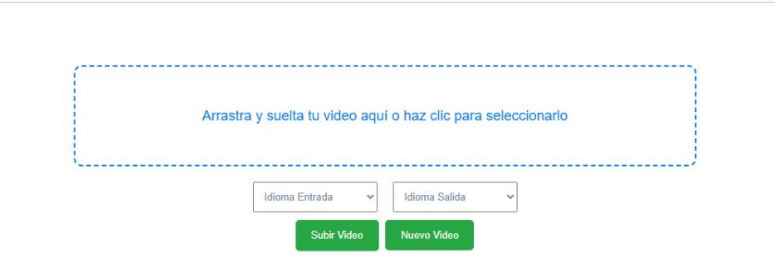
\includegraphics[width=13.4cm]{\audio}}}\\
    \hline
    \cellcolor{bleudefrance}\textbf{\color{aliceblue} Desarrollador:} 
    & \multicolumn{4}{|l|}{GUZMAN HONOR WILSON} \\
    \hline
    \rowcolor{bleudefrance}\multicolumn{5}{|c|}{ }\\
    \hline

\end{longtable}